\subsubsection{Proceso: Realizar gráfica 2D}

\begin{itemize}
	\item \textbf{O1:} Busca los valores de los atributos a partir del nombre y del nombre del juego, y consigue la tupla fecha, valor, nombre de jugador.
\end{itemize}

\begin{figure}[H]
	\centering
	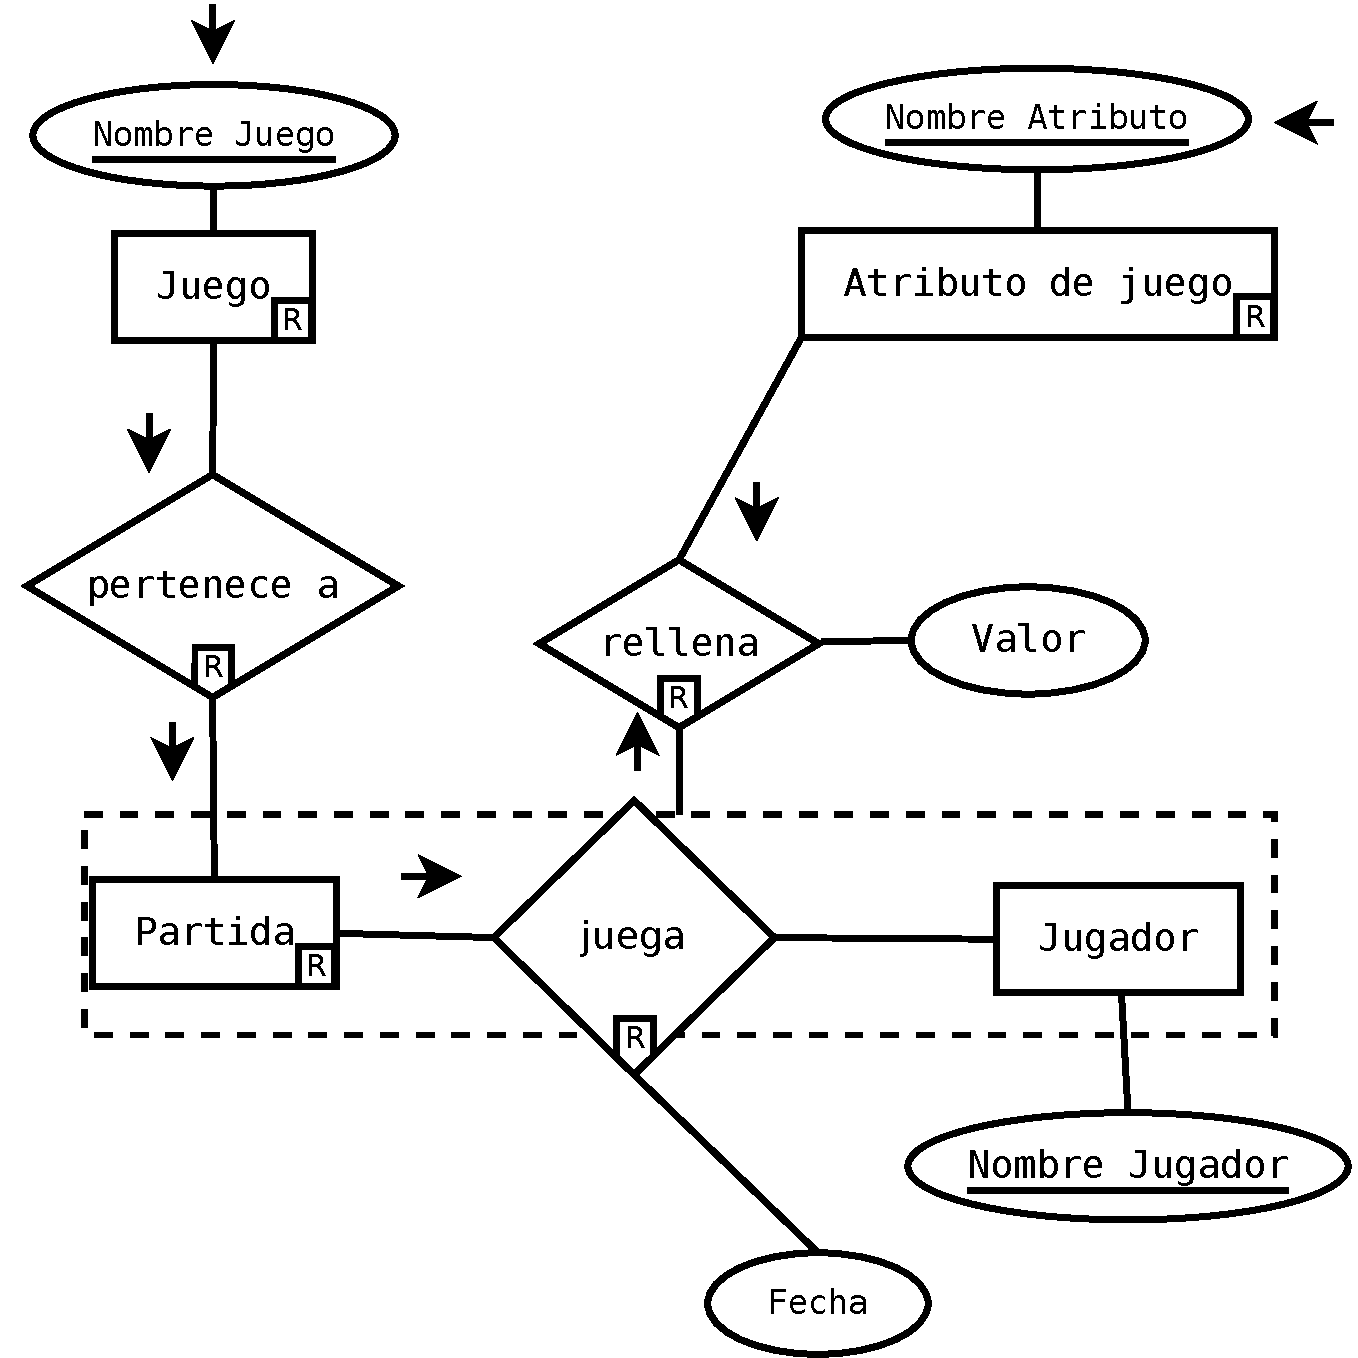
\includegraphics[width=0.5\linewidth]{../Diagramas/pdf/OpEstadisticas3.pdf}
	\caption{Esquema de navegabilidad  O1 del proceso 4.1}
	
	\label{fig:O4.1}
\end{figure}
 \begin{itemize}
 	\item \textbf{O2:} Con los valores anteriores, se ha realizado una gráfica 2D que con esta operación insertamos. Conseguimos el usuario que está haciendo la estadística, la imagen de ella y su id, y la insertamos de forma correcta en la base de datos.
 \end{itemize}

\begin{figure}[H]
	\centering
	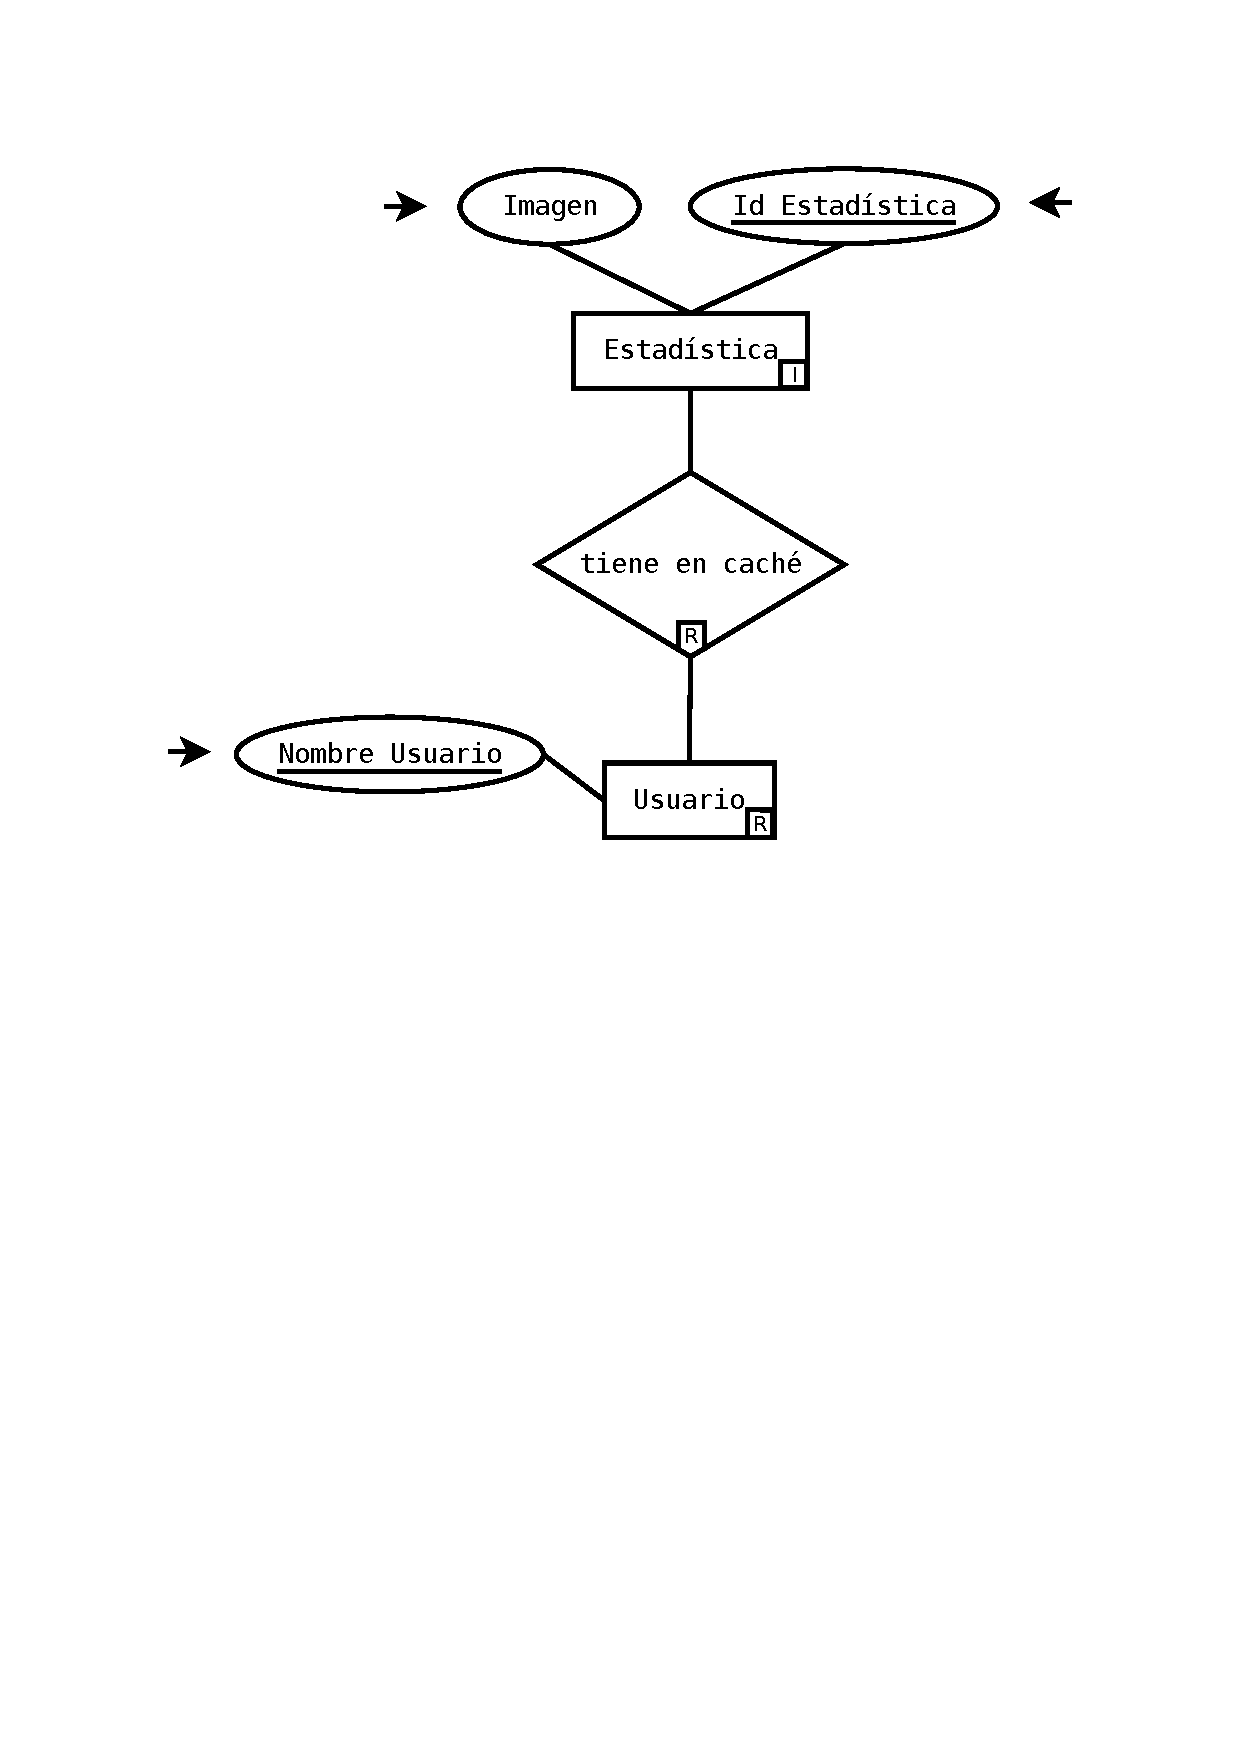
\includegraphics[width=0.5\linewidth]{../Diagramas/pdf/OpEstadisticas1-2.pdf}
	\caption{Esquema de navegabilidad  O2 del proceso 4.1}
	
	\label{fig:O4.12}
\end{figure}

\subsubsection{Proceso: Realizar gráfica 3D}

\begin{itemize}
	\item \textbf{O1:} Busca los valores de los atributos a partir del nombre y del nombre del juego, y consigue la tupla fecha, valor, nombre de jugador.
\end{itemize}

\begin{figure}[H]
	\centering
	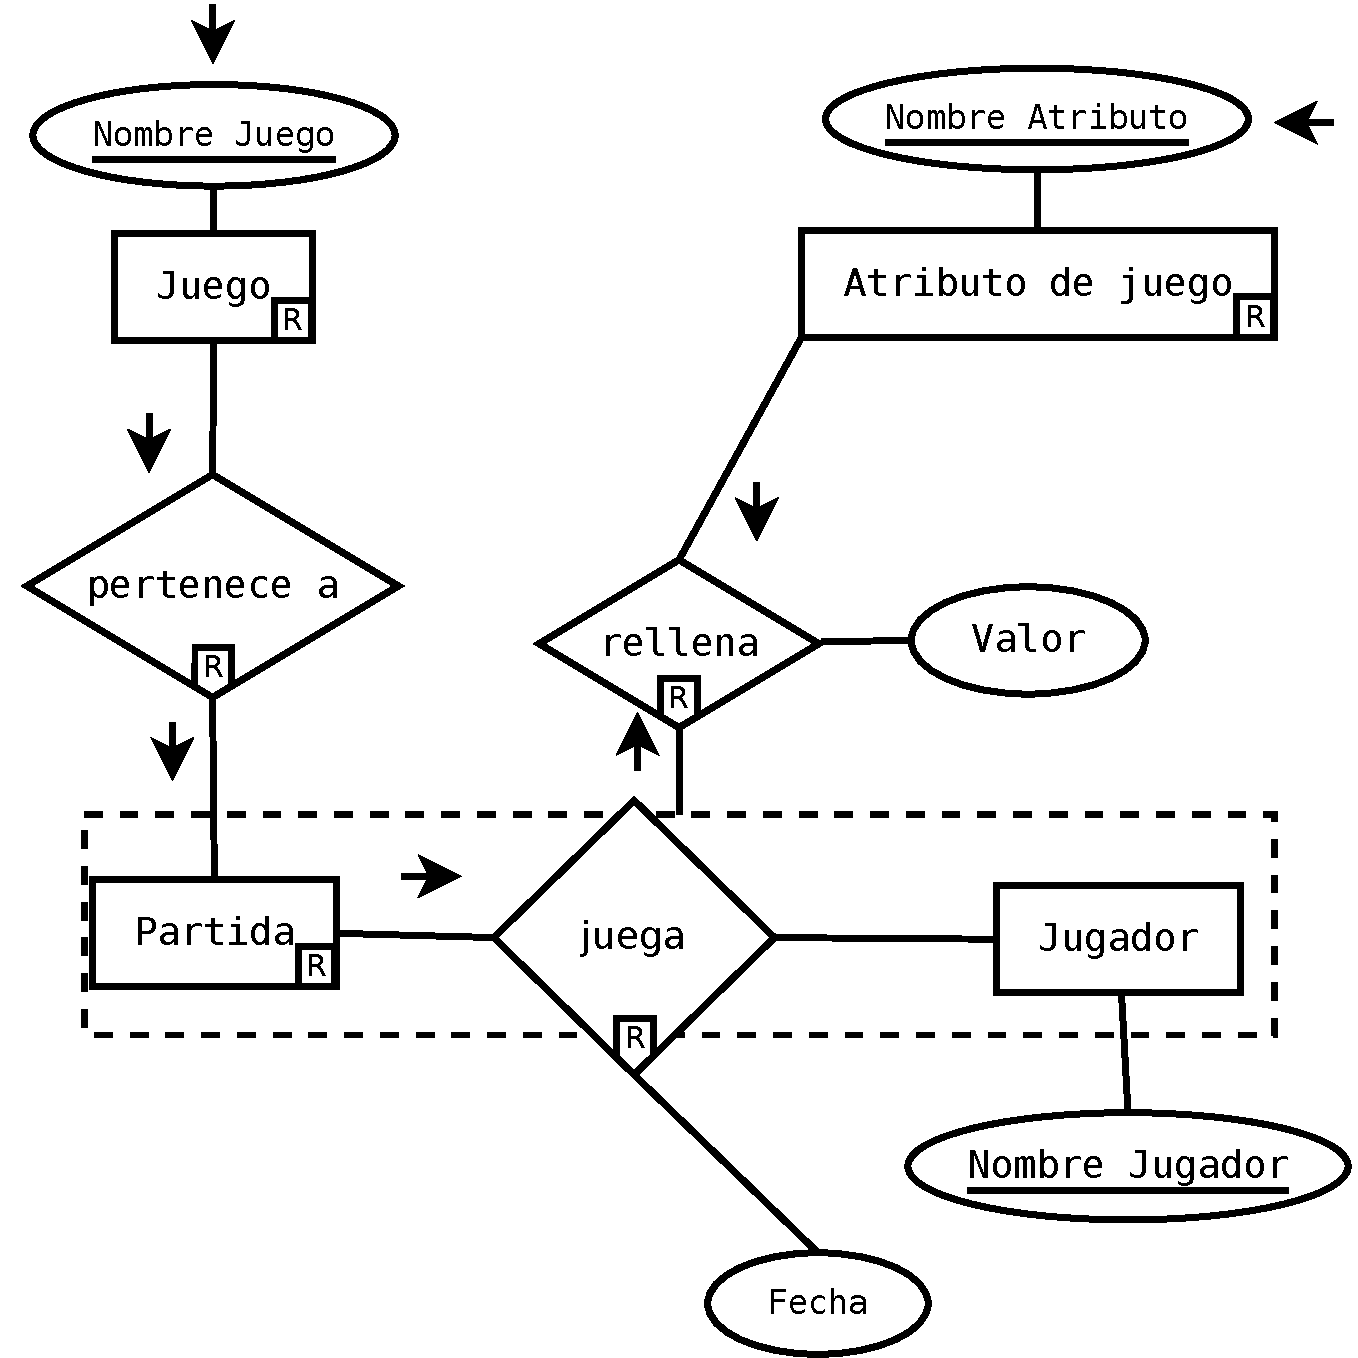
\includegraphics[width=0.5\linewidth]{../Diagramas/pdf/OpEstadisticas3.pdf}
	\caption{Esquema de navegabilidad  O1 del proceso 4.2}
	
	\label{fig:O4.2}
\end{figure}
\begin{itemize}
	\item \textbf{O2:} Con los valores anteriores, se ha realizado una gráfica 3D que con esta operación insertamos. Conseguimos el usuario que está haciendo la estadística, la imagen de ella y su id, y la insertamos de forma correcta en la base de datos.
\end{itemize}

\begin{figure}[H]
	\centering
	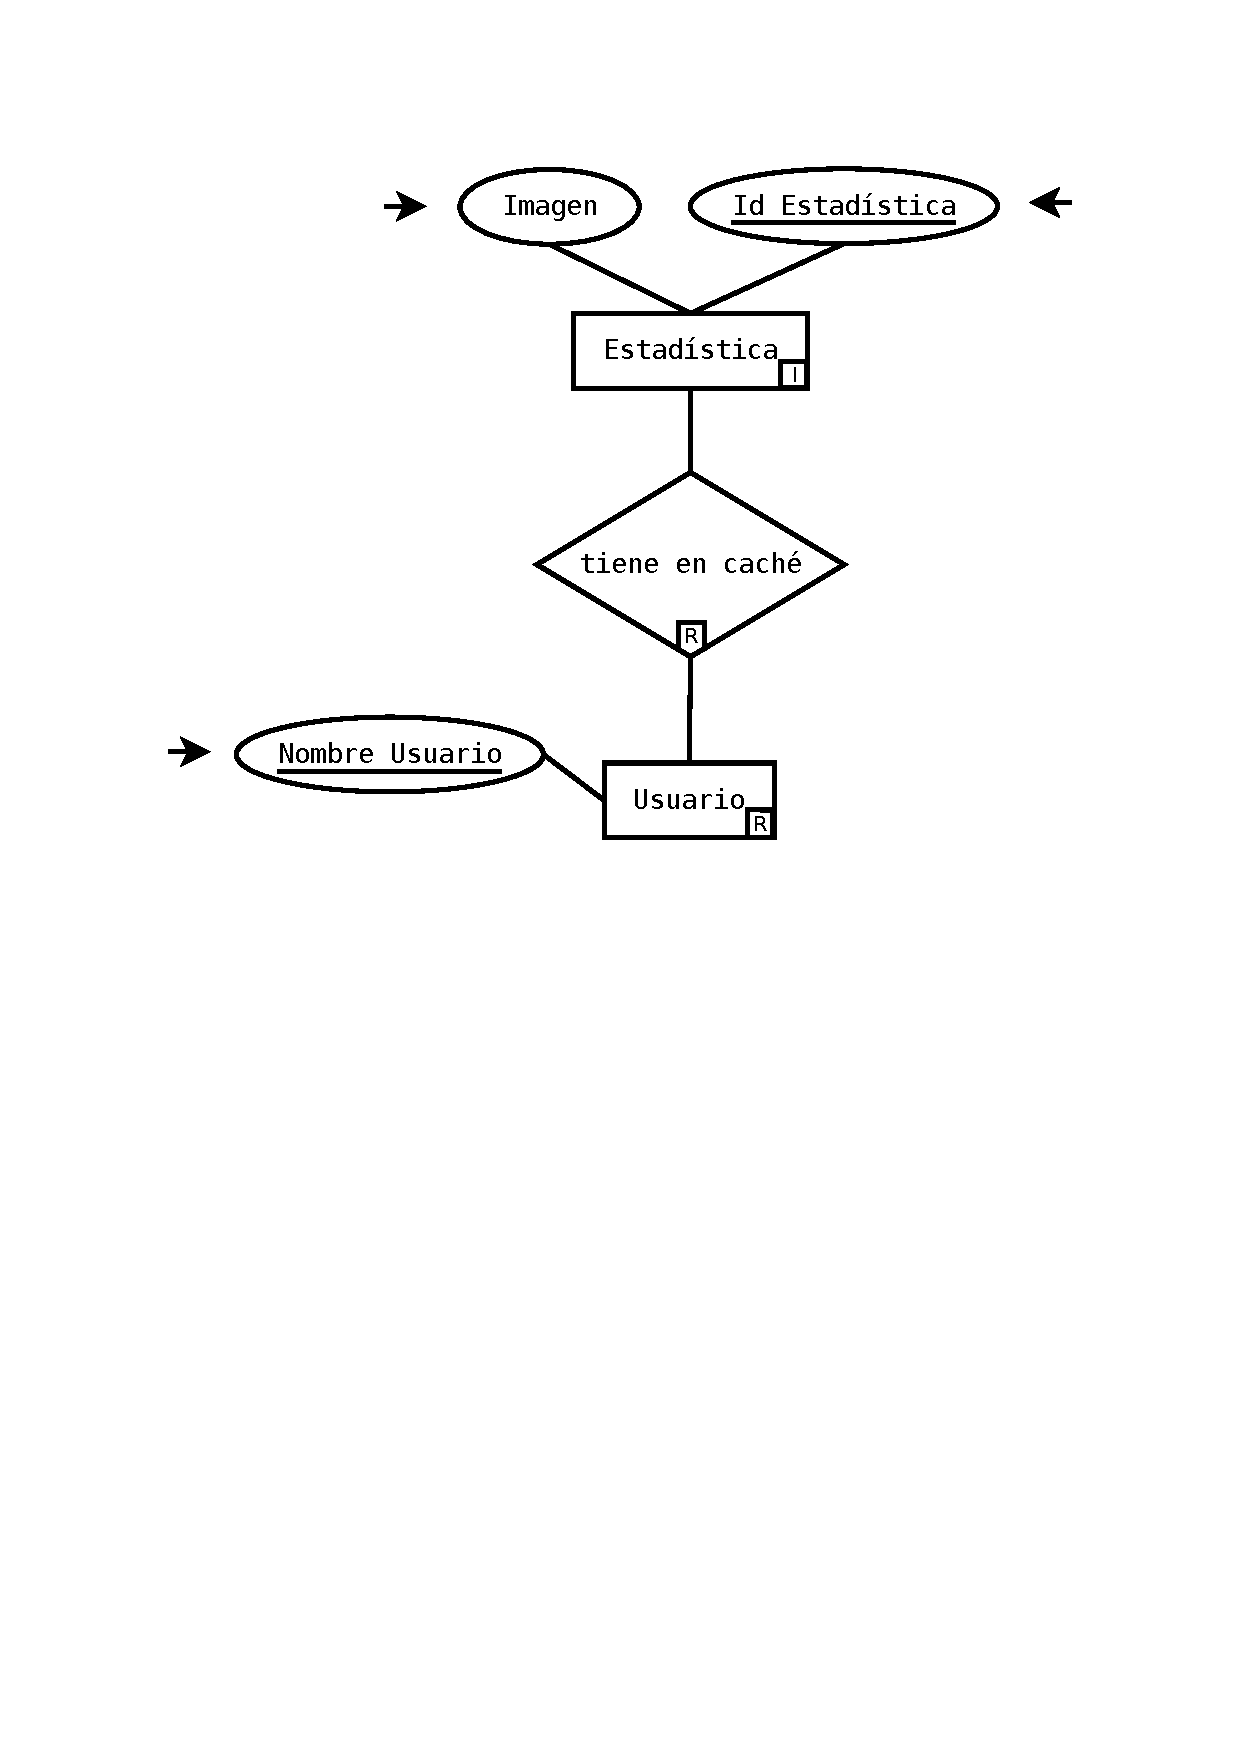
\includegraphics[width=0.5\linewidth]{../Diagramas/pdf/OpEstadisticas1-2.pdf}
	\caption{Esquema de navegabilidad  O2 del proceso 4.2}
	
	\label{fig:O4.22}
\end{figure}

\subsubsection{Proceso: Realizar gráfica de columnas agrupadas}

\begin{itemize}
	\item \textbf{O1:} Busca los valores de los atributos a partir del nombre y del nombre del juego, y consigue la tupla fecha, valor, nombre de jugador.
\end{itemize}

\begin{figure}[H]
	\centering
	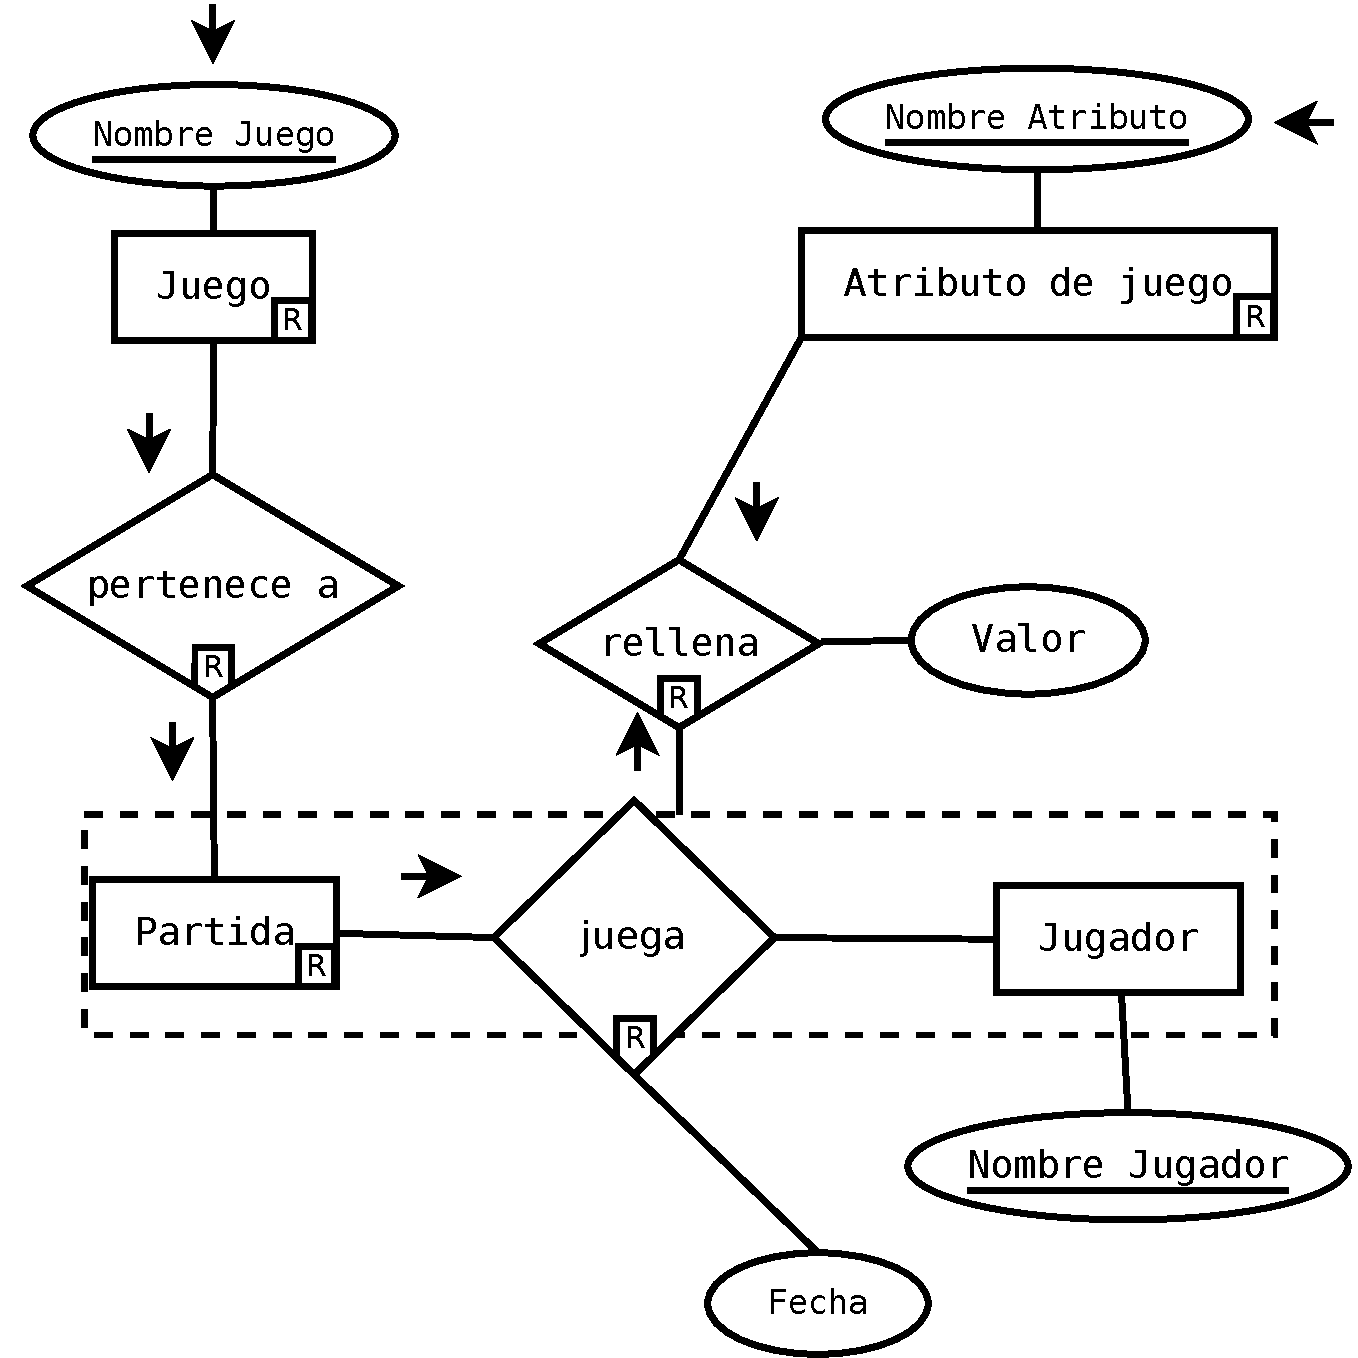
\includegraphics[width=0.5\linewidth]{../Diagramas/pdf/OpEstadisticas3.pdf}
	\caption{Esquema de navegabilidad  O1 del proceso 4.3}
	
	\label{fig:O4.3}
\end{figure}
\begin{itemize}
	\item \textbf{O2:} Con los valores anteriores, se ha realizado una gráfica de columnas agrupadas que con esta operación insertamos. Conseguimos el usuario que está haciendo la estadística, la imagen de ella y su id, y la insertamos de forma correcta en la base de datos.
\end{itemize}

\begin{figure}[H]
	\centering
	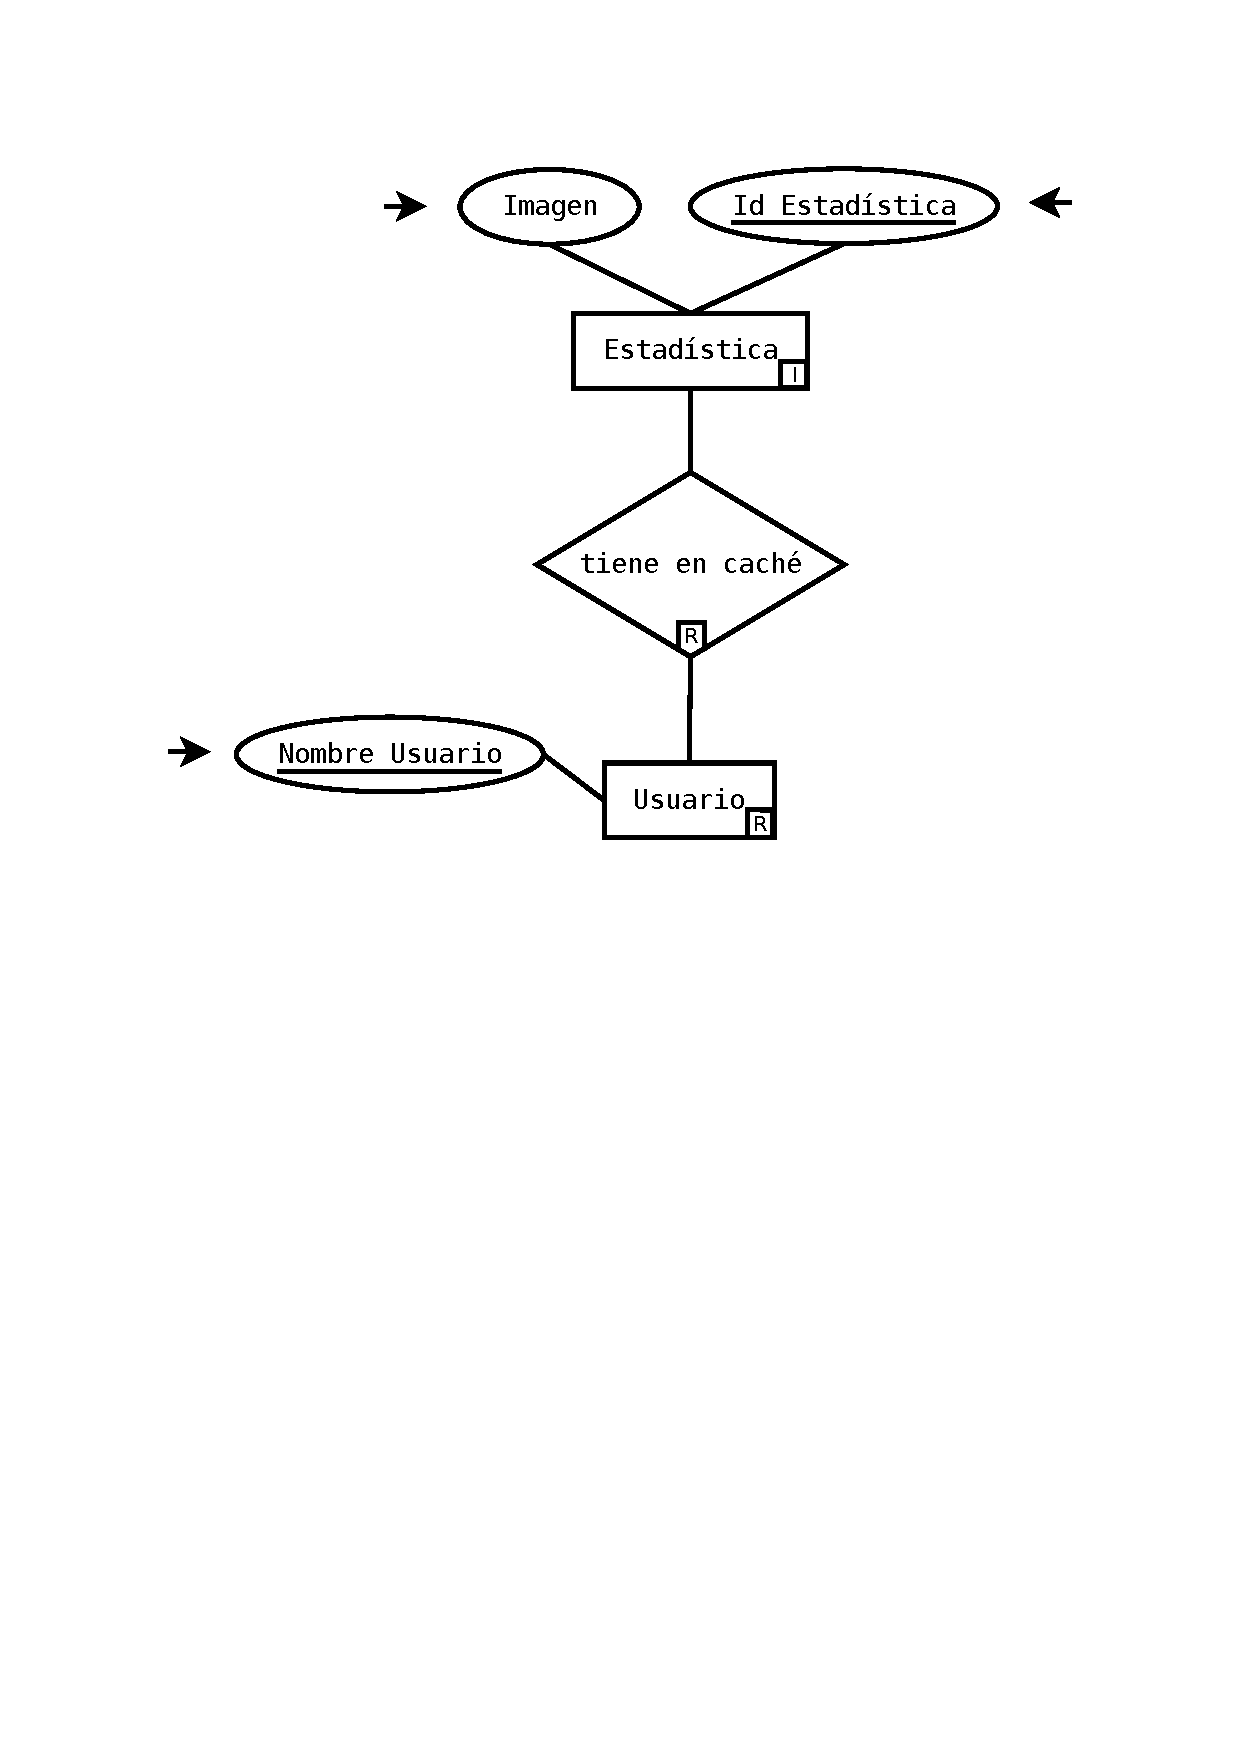
\includegraphics[width=0.5\linewidth]{../Diagramas/pdf/OpEstadisticas1-2.pdf}
	\caption{Esquema de navegabilidad  O2 del proceso 4.3}
	
	\label{fig:O4.32}
\end{figure}


\subsubsection{Proceso: Realizar gráfica circular}

\begin{itemize}
	\item \textbf{O1:} Busca los valores de los atributos a partir del nombre y del nombre del juego, y consigue la tupla fecha, valor, nombre de jugador.
\end{itemize}

\begin{figure}[H]
	\centering
	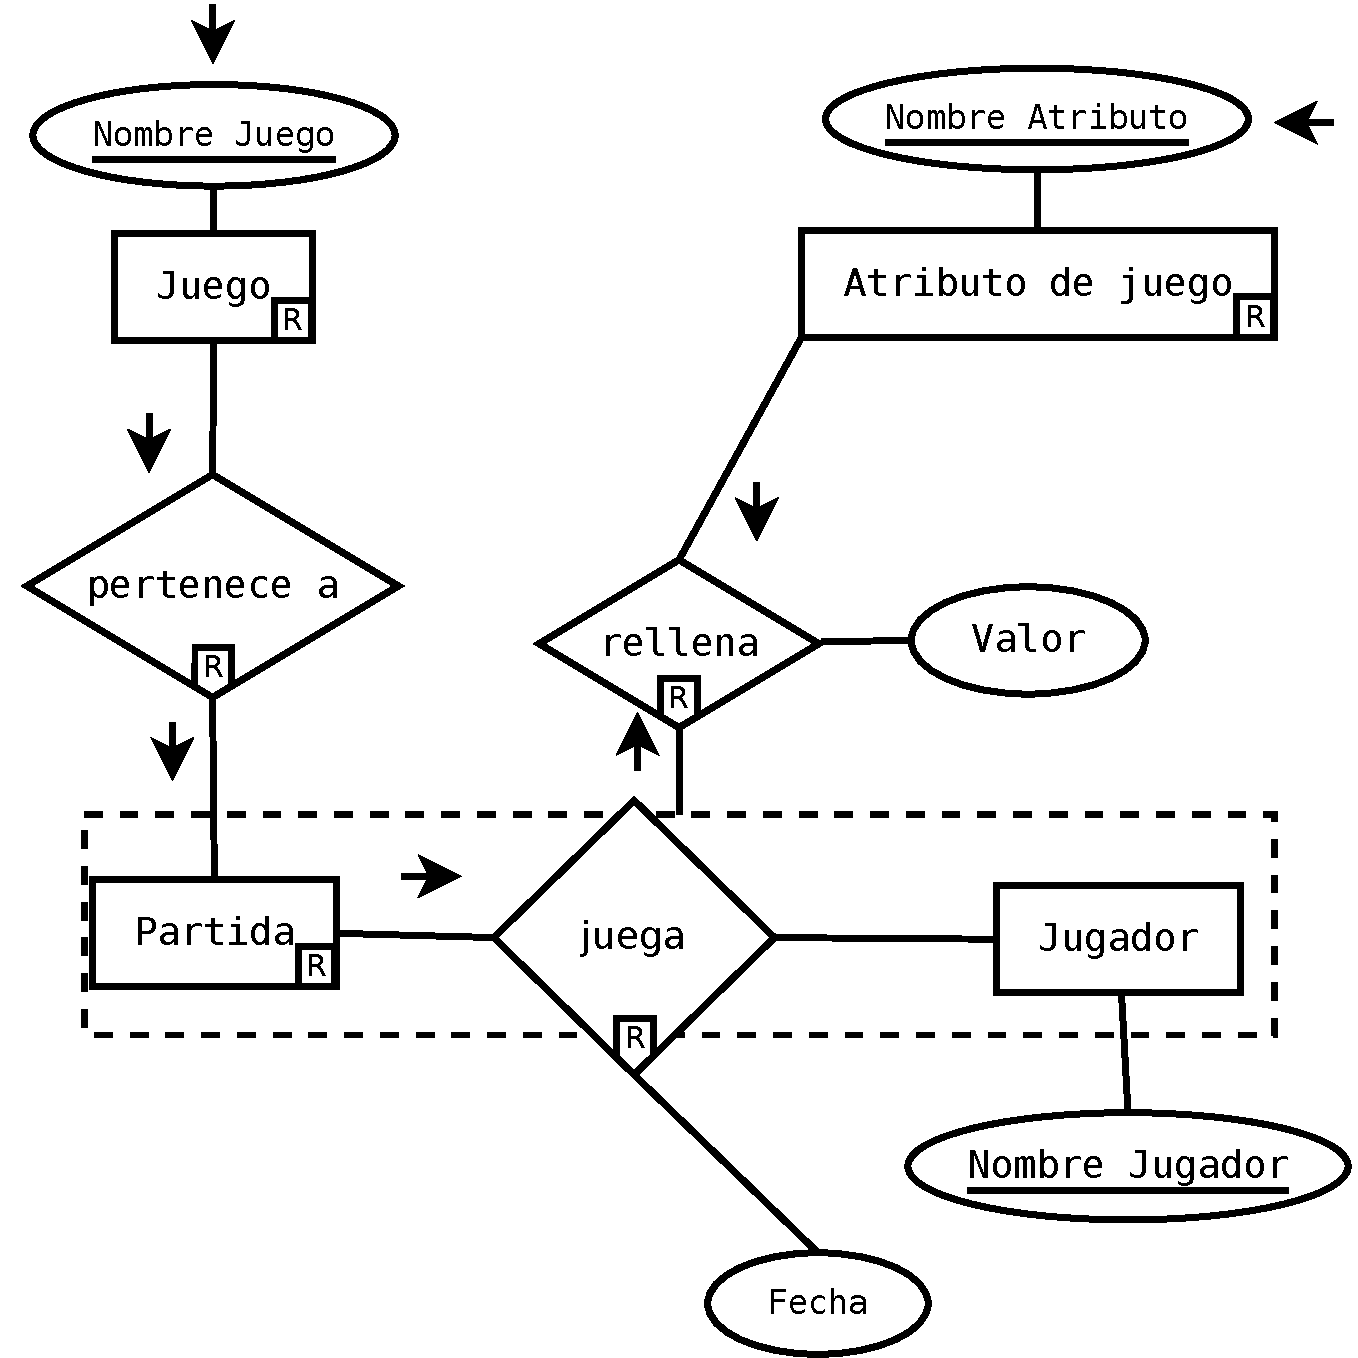
\includegraphics[width=0.5\linewidth]{../Diagramas/pdf/OpEstadisticas3.pdf}
	\caption{Esquema de navegabilidad  O1 del proceso 4.4}
	
	\label{fig:O4.4}
\end{figure}
\begin{itemize}
	\item \textbf{O2:} Con los valores anteriores, se ha realizado una gráfica circular que con esta operación insertamos. Conseguimos el usuario que está haciendo la estadística, la imagen de ella y su id, y la insertamos de forma correcta en la base de datos.
\end{itemize}

\begin{figure}[H]
	\centering
	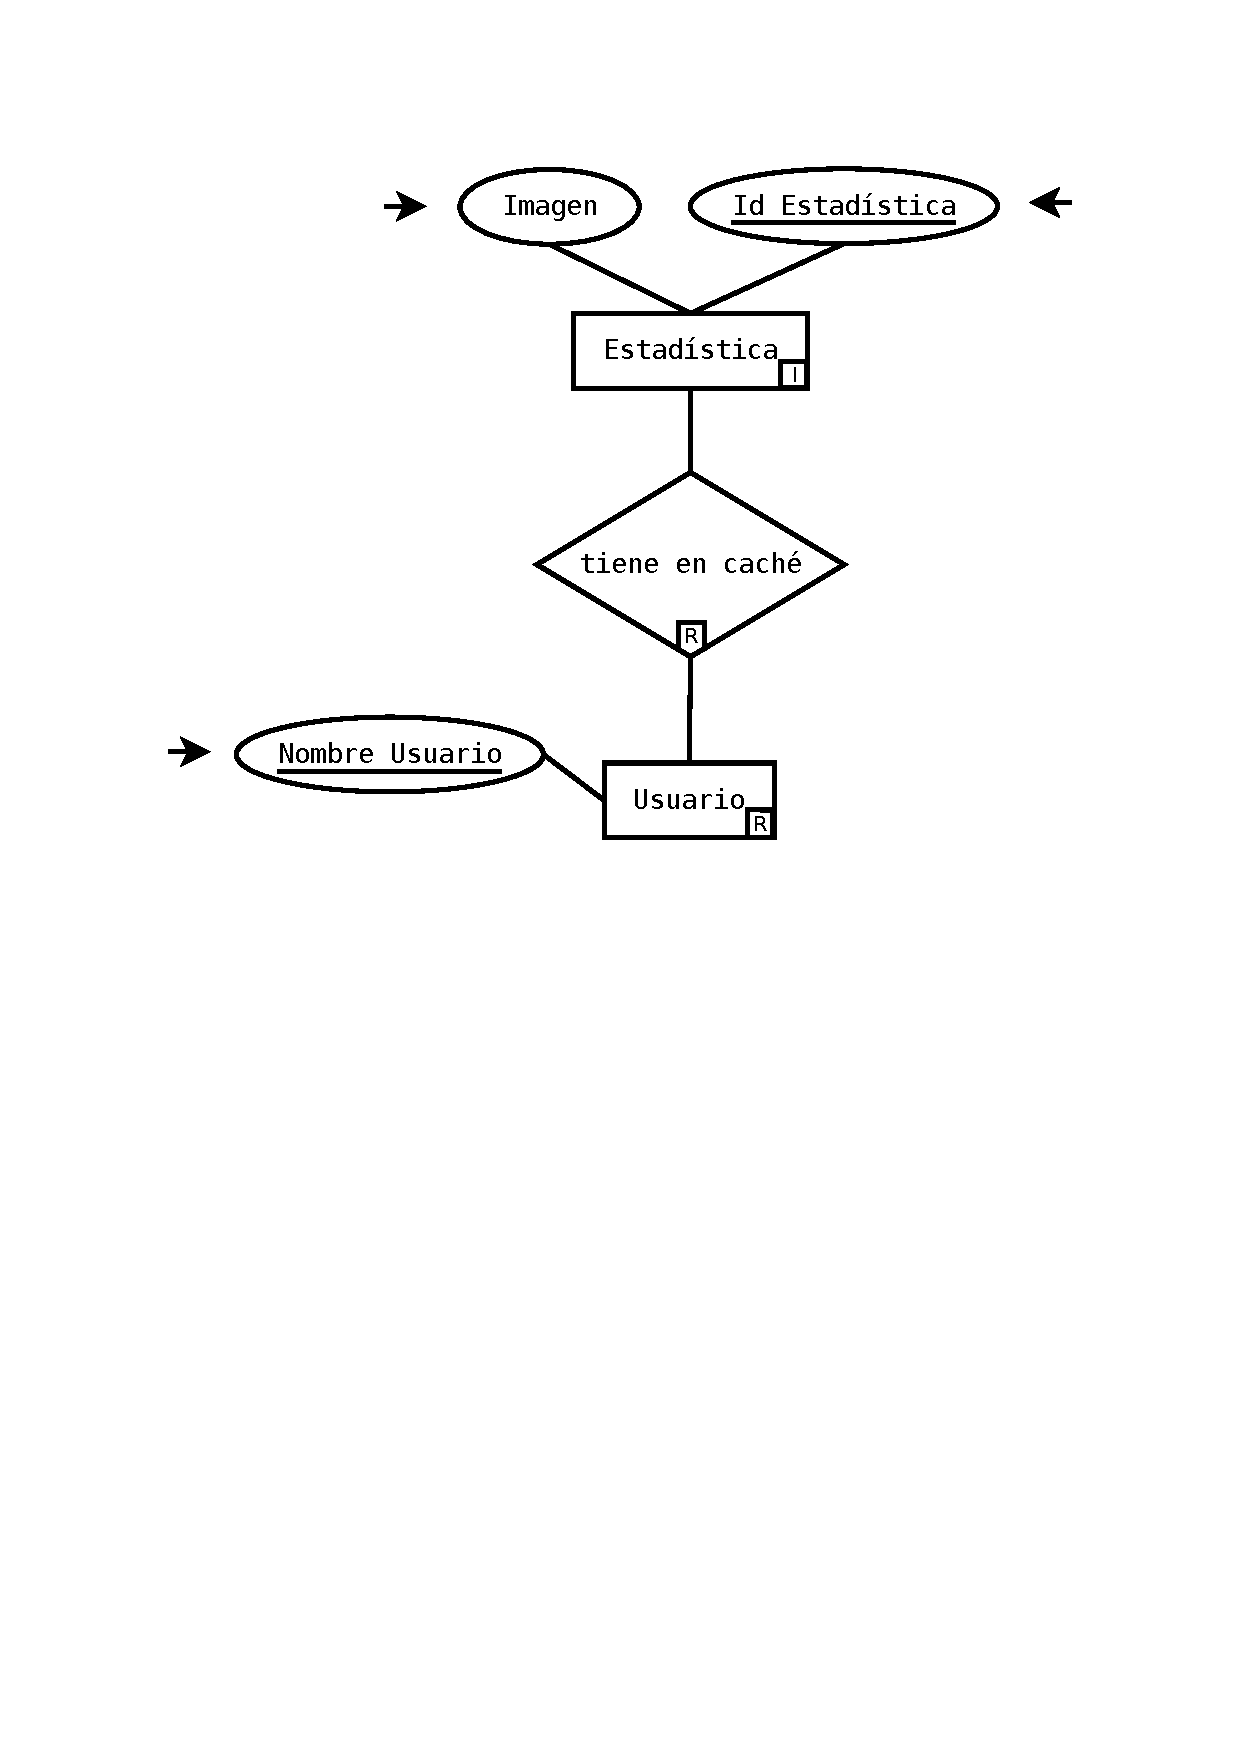
\includegraphics[width=0.5\linewidth]{../Diagramas/pdf/OpEstadisticas1-2.pdf}
	\caption{Esquema de navegabilidad  O2 del proceso 4.4}
	
	\label{fig:O4.42}
\end{figure}

\subsubsection{Proceso: Realizar función de un atributo}

\begin{itemize}
	\item \textbf{O1:} Buscamos, a partir del nombre del juego y del nombre del atributo, los valores que los relacionan. En este caso como trabajamos con todas las partidas por igual no necesitaremos los valores adicionales de fecha y nombre del jugador.
\end{itemize}

\begin{figure}[H]
	\centering
	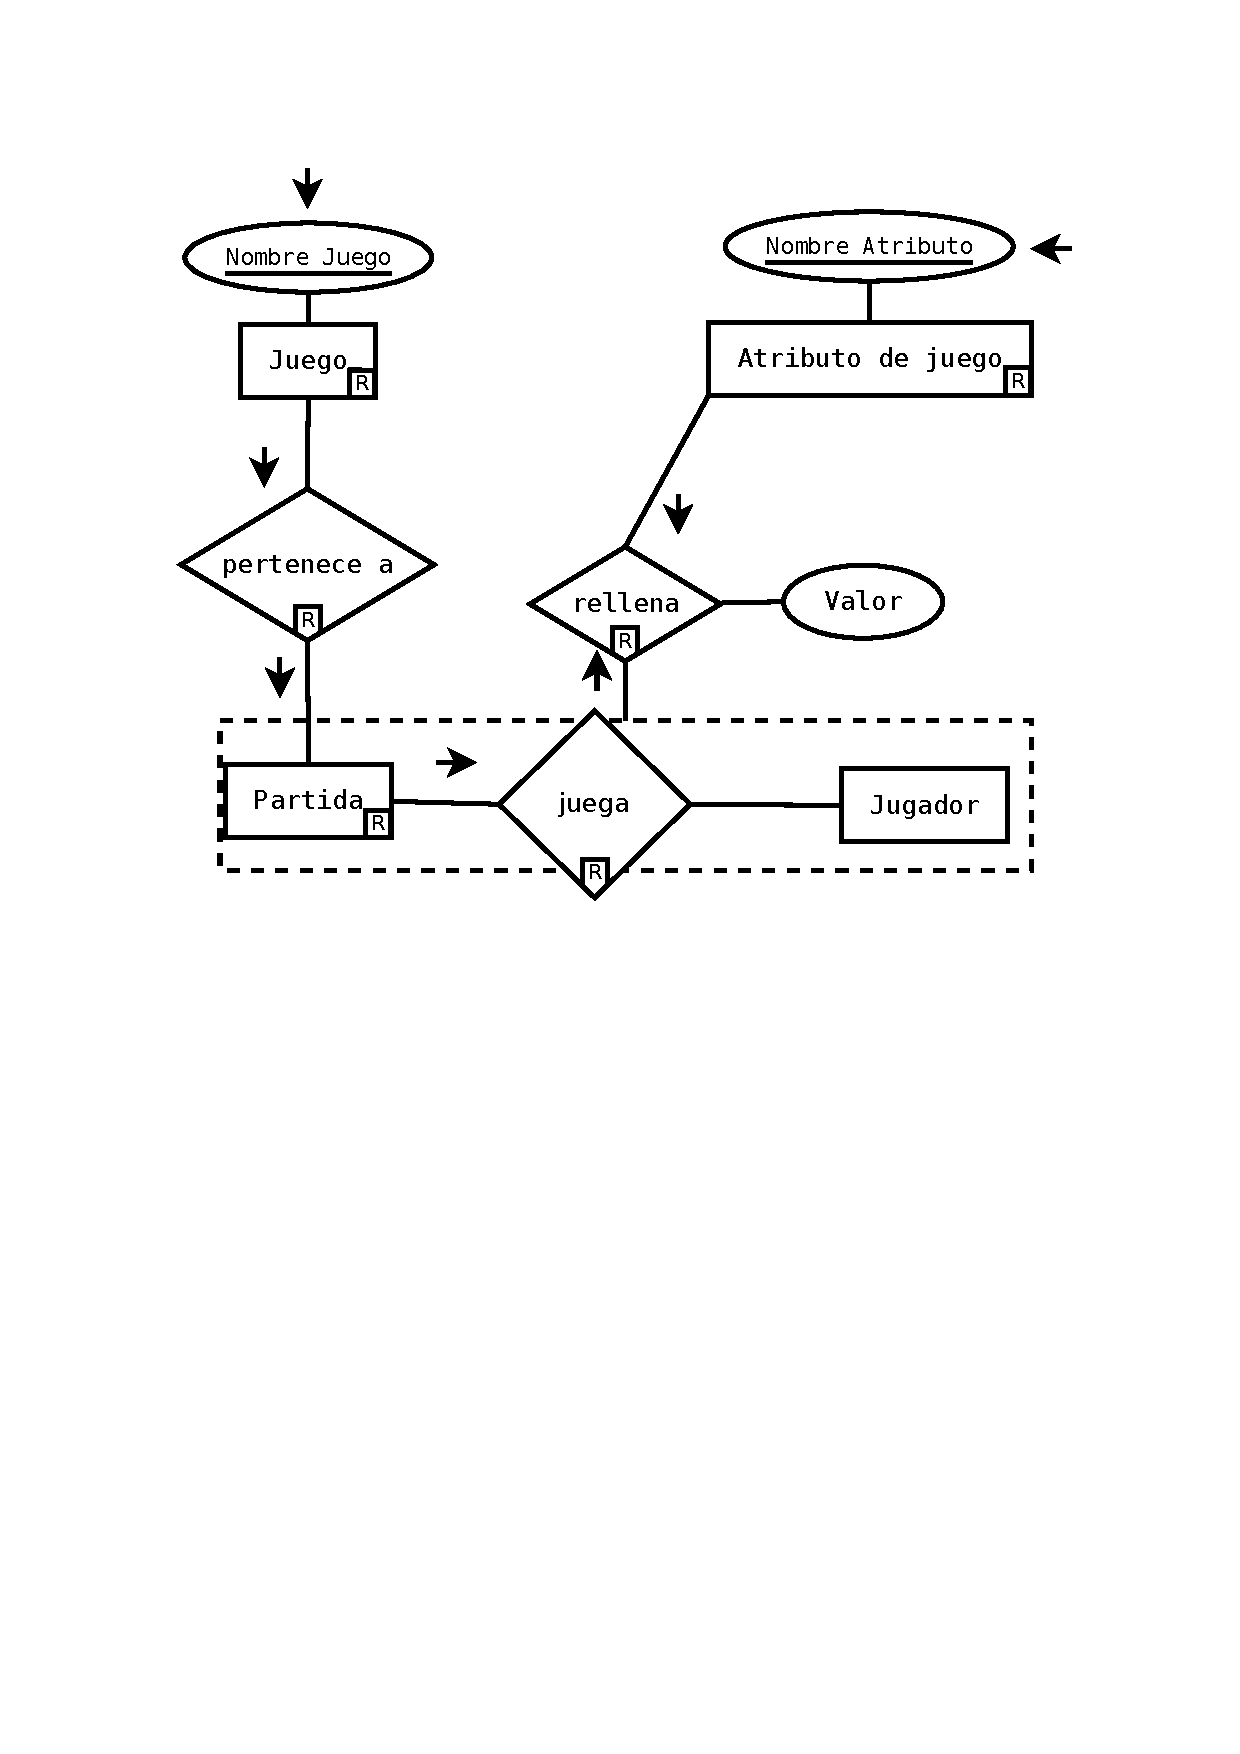
\includegraphics[width=0.5\linewidth]{../Diagramas/pdf/OpEstadisticas5.pdf}
	\caption{Esquema de navegabilidad  O1 del proceso 4.5}
	
	\label{fig:O4.5}
\end{figure}

Después de esto el proceso debería realizar la función correspondiente y devolverla, pero eso no afecta a la base de datos.

\subsubsection{Proceso: Conseguir las últimas gráficas pedidas}

\begin{itemize}
	\item \textbf{O1: A partir del nombre de usuario conseguimos las imágenes de estadísticas que están relacionadas con él a partir de la relación tiene en caché.} 
\end{itemize}

\begin{figure}[H]
	\centering
	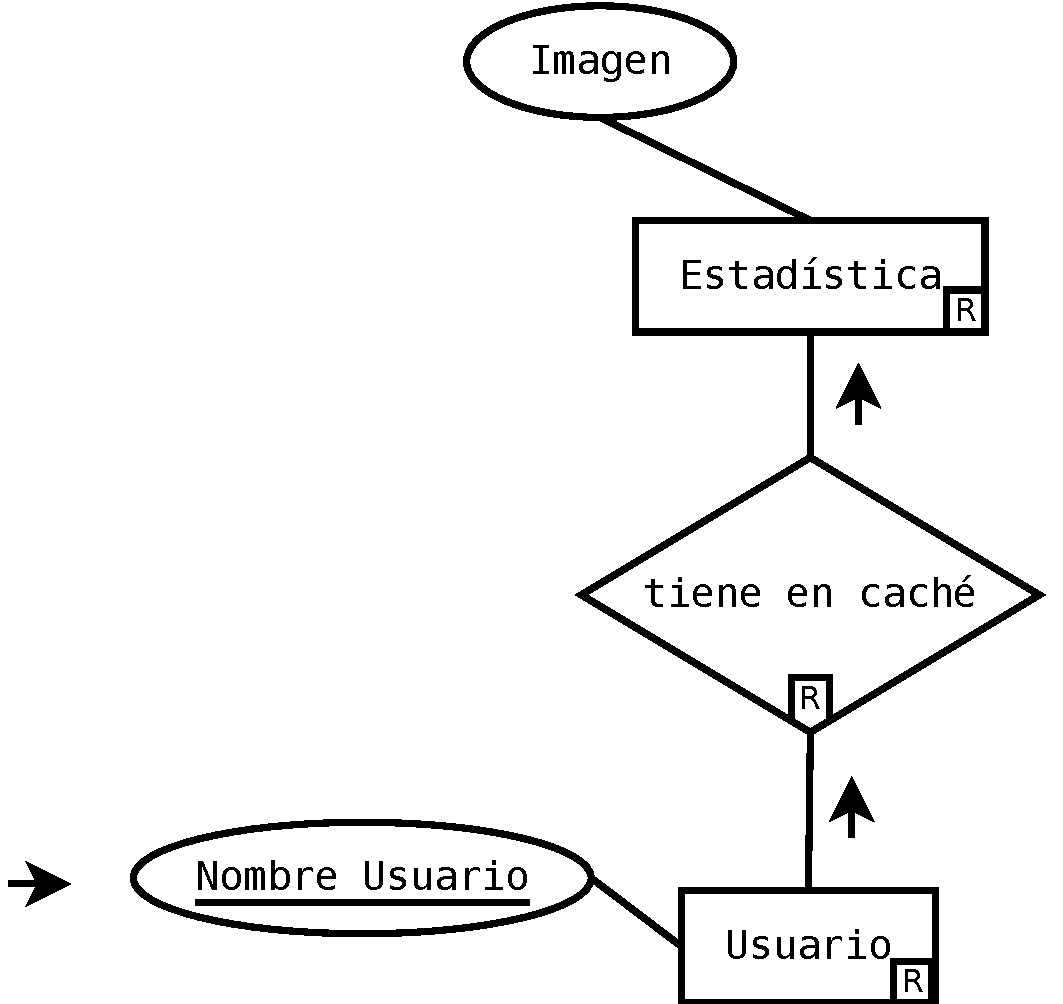
\includegraphics[width=0.5\linewidth]{../Diagramas/pdf/OpEstadisticas6.pdf}
	\caption{Esquema de navegabilidad  O1 del proceso 4.6}
	
	\label{fig:O4.6}
\end{figure}

Después de esto el programa debería devolver estas estadísticas como imagen al usuario.
